\chapter{Идентификация имплантируемых роторных насосов крови в аппаратах вспомогательного кровообращения} \label{chapt1}

Цель данной главы заключается в рассмотрении истории развития имплантируемых роторных насосов крови, а также проблемы идентификации данных насосов в аппаратах вспомогательного кровообращения. 

% роторного насоса крови, а также обзоре и сравнительном анализе различных способов идентификации имплантируемым роторным насосом крови в аппаратах вспомогательного кровообращения. 

%Аппараты вспомогательного кровообращения (АВК) успешно применяются в качестве альтернативы трансплантации сердца при лечении тяжелых форм сердечной недостаточности \cite{Patel2014667,Mancini_2015,HT_LVAD_2013,Lima2015360,Schumerehv590,ottenberg_choices_2014,selzman_bridge_2015,drakos_clinical_2016}.

%\section{Идентификация имплантируемого роторного насоса крови} \label{sect_1_1}

\section{История развития имплантируемых роторных насосов крови в аппаратах вспомогательного кровообращения} \label{chapt1_history}

Сердечная недостаточность является тяжелым, прогрессирующим заболеванием, которое характеризуется неспособностью сердца перекачивать кровь в объеме, достаточном для обеспечения метаболических потребностей организма. Около восьми миллионов человек страдают от хронической сердечной недостаточности в России и около 5 миллионов -- в США, из которых ежегодно умирает около 900 тысяч в России и примерно 300 тысяч в США. Сердечная недостаточность является самой распространенной причиной госпитализации в стационары и смерти от сердечно-сосудистых заболеваний \cite{debakey2000odyssey, starling2011potential, ponikowski2014heart, wong2014epidemiological, selishchev2015ventricular}. 

Под сердечной недостаточностью наиболее часто подразумевают недостаточность левого желудочка сердца. Правожелудочковая недостаточность чаще наблюдается как вторичная по отношению к левожелудочковой недостаточности. Легкая сердечная недостаточность проявляется сниженной способностью переносить физическую нагрузку и развитием одышки во время физической активности. При более тяжелых формах пациент может фактически не иметь способности переносить физическую нагрузку и испытывать одышку в состоянии покоя. 
% 
% Если там их число ежегодно колеблется около двух тысяч, то у нас — около ста. Однако ни то, ни другое число даже близко не приближается к числу больных, которые нуждаются в таких трансплантациях. В США по этой причине каждый год умирает по 55 тысяч человек, в России — 110 тысяч. Вряд ли проблема доступности донорских сердец будет решена в обозримом будущем, поэтому нужда в системах вспомогательного кровообращения выходит на первое место.
% 
% Система вспомогательного кровообращения при всем многообразии ее разновидностей представляет собой, грубо говоря, насос, который гонит кровь, заменяя собой правый или левый желудочек сердца. Естественно, не все так просто: этот насос должен удовлетворять массе требований, важнейшие из которых — он должен работать со стопроцентной надежностью и не «портить» кровь, не разрушать ее элементы.

Сердечная недостаточность может являться результатом ухудшенной сократительной способности сердечной мышцы (систолическая недостаточность) или нарушенного наполнения сердца (диастолическая недостаточность). Оба механизма сердечной недостаточности можно описать с помощью контуров давление-объем желудочка сердца, представленных на рисунке \ref{img:pv_loops}. 

% \begin{figure}[ht] 
%   \center
%   \includegraphics [width=\textwidth] {../images/c1_pv_loops_failure}
%   \caption{} 
%   \label{img:}  
% \end{figure}

\begin{figure}[ht]
  \begin{minipage}[ht]{0.32\linewidth}
    \center{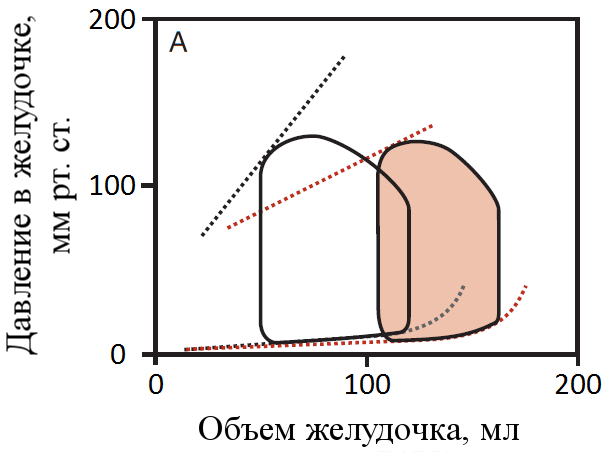
\includegraphics [scale=0.3] {../images/c1_pv_loop_systolic} \\ а)}
  \end{minipage}
  \hfill
  \begin{minipage}[ht]{0.32\linewidth}
    \center{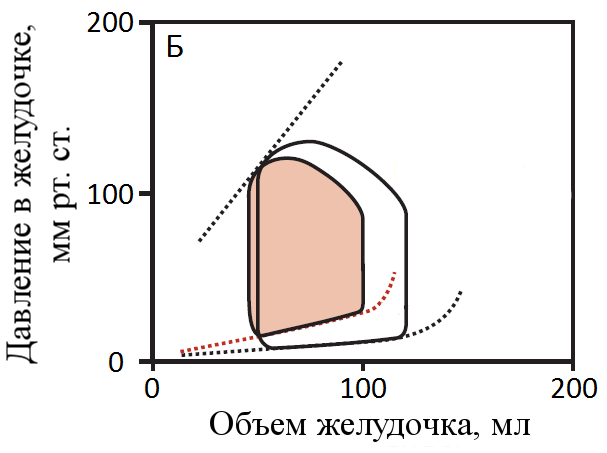
\includegraphics [scale=0.3] {../images/c1_pv_loop_diastolic} \\ б)}
  \end{minipage}
  \hfill
  \begin{minipage}[ht]{0.32\linewidth}
    \center{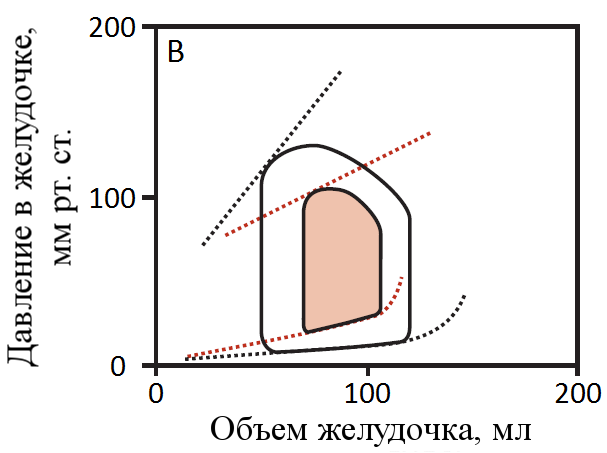
\includegraphics [scale=0.3] {../images/c1_pv_loop_comb} \\ в)}
  \end{minipage}
  \caption{Влияние систолической (а) диастолической (б) и комбинированной (в) сердечной недостаточности на контуры давление-объем желудочка сердца}
  \label{img:pv_loops}  
\end{figure}

При систолической недостаточности сердце выбрасывает меньший объем крови, что приводит к увеличению конечно-систолического объема желудочка сердца и сдвигу контура вправо -- рисунок \ref{img:pv_loops}а.

Второй тип сердечной недостаточности -- диастолическая недостаточность -- обусловлен нарушенным наполнением желудочка вследствие либо уменьшения степени растяжимости желудочка, либо нарушением релаксации. Так, снижение степени растяжимости приводит к уменьшению объема крови в желудочке и повышению диастолического давления -- контур давление-объем сдвигается влево и его площадь уменьшается. 

Хроническая сердечная недостаточность зачастую характеризуется сочетанием как систолического, так и диастолического нарушений разной степени тяжести -- рисунок \ref{img:pv_loops}в.

В настоящее время золотым стандартом лечения тяжелых форм сердечной недостаточности является трансплантация сердца. В мире ежегодно выполняется около 3500 трансплантаций, из которых примерно 2400 в США и около 100 в России \cite{frazier2017invited, transpl_ru}. Тем не менее, возможности трансплантации ограничены вследствие недостатка донорских органов и наличия целого ряда противопоказаний для пересадки. Кроме того, трансплантация требует дорогостоящей иммуносупрессивной терапии и постоянных обследований после операции. 

Альтернативной трансплантации сердца является имплантация аппаратов вспомогательного кровообращения (АВК), предназначенных для частичной или полной замены функции, как правило, левого желудочка сердца \cite{Patel2014667, Mancini_2015, HT_LVAD_2013, daners2017left}. Данный способ хирургического лечения сердечной недостаточности получил активное развитие в последние десять лет -- в настоящее время ежегодно осуществляется около 2500 имплантаций \cite{kirklin2015seventh}.

АВК могут использоваться для краткосрочной поддержки кровообращения у пациентов, ожидающих трансплантации донорского органа, для продолжительной поддержки на протяжении многих лет у пациентов, которым было отказано в трансплантации, либо для восстановления сократительной функции их собственного сердца \cite{ottenberg_choices_2014, selzman_bridge_2015, drakos_clinical_2016, wever2016cardiac}. 

Основной частью АВК является роторный насос крови (РНК), который имплантируется в грудную клетку пациента и соединяется при помощи чрескожного кабеля с системой управления.

Самые первые насосы пульсирующего типа появились в конце 70-х годов двадцатого века. Они представляли собой искусственные желудочки сердца с подвижной мембраной, обеспечивающей пульсирующий поток. В то время распространенной была гипотеза о том, что аппараты вспомогательного кровообращения должны имитировать работу биологического сердца \cite{frazier2017invited}. Среди основных насосов пульсирующего типа следует выделить, EXCOR Berlin Heart и HeartMate I, представленный на рисунке \ref{img:heartmate_one}. Аппараты вспомогательного кровообращения с насосом HeartMate I начали успешно имплантироваться с 1991 года, позволяя пациентам покинуть больницу.

\begin{figure}[ht] 
  \center
  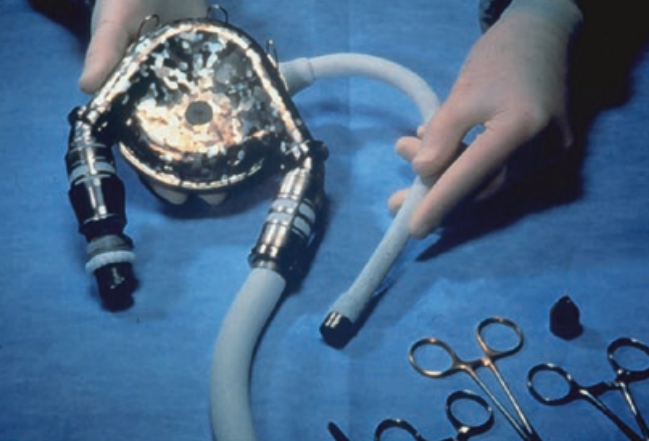
\includegraphics [width=0.6\textwidth] {../images/c1_heartmate_one}
  \caption{Насос пульсирующего типа HeartMate I \cite{frazier2017invited}} 
  \label{img:heartmate_one}  
\end{figure}

В то же время данные аппараты характеризовались невысокой надежностью по причине использования мембраны и требовали замены примерно каждые два года. Кроме того, они обладали большими размерами, не позволявшими имплантировать их женщинам и детям \cite{frazier2017invited}. 

\subsection*{Имплантируемые роторные насосы крови} \label{chapt1_irbps}

Следующим этапом развития технологии вспомогательного кровообращения стало появление роторных насосов крови \cite{reul2000blood, daners2017left}, обусловленное потребностью в продолжительной поддержке кровообращения \cite{frazier2017invited}.

Перекачивание крови в роторных насосах происходит посредством вращения рабочего колеса (ротора), создающего градиент давлений на входе и выходе насоса и обеспечивающего непрерывное течение жидкости. Ротор с постоянным магнитом внутри приводится во вращение за счет изменения магнитного поля, создаваемого статором \cite{nose1998design, mt2010n6_ru}. На входе в насос расположен направляющий аппарат (диффузор) с опорами из износостойкого материала, на выходе -- спрямляющий аппарат, в котором так же установлены опоры для ротора. Описанные компоненты образуют проточную часть насоса. Пример проточной части роторного насоса крови Спутник представлен на рисунке \ref{img:pump_view}а. Геометрия данной части насоса проектируется таким образом, чтобы добиться минимальной травмы крови с учетом высокой скорости вращения ротора насоса.

% \begin{figure}[ht] 
%   \center
%   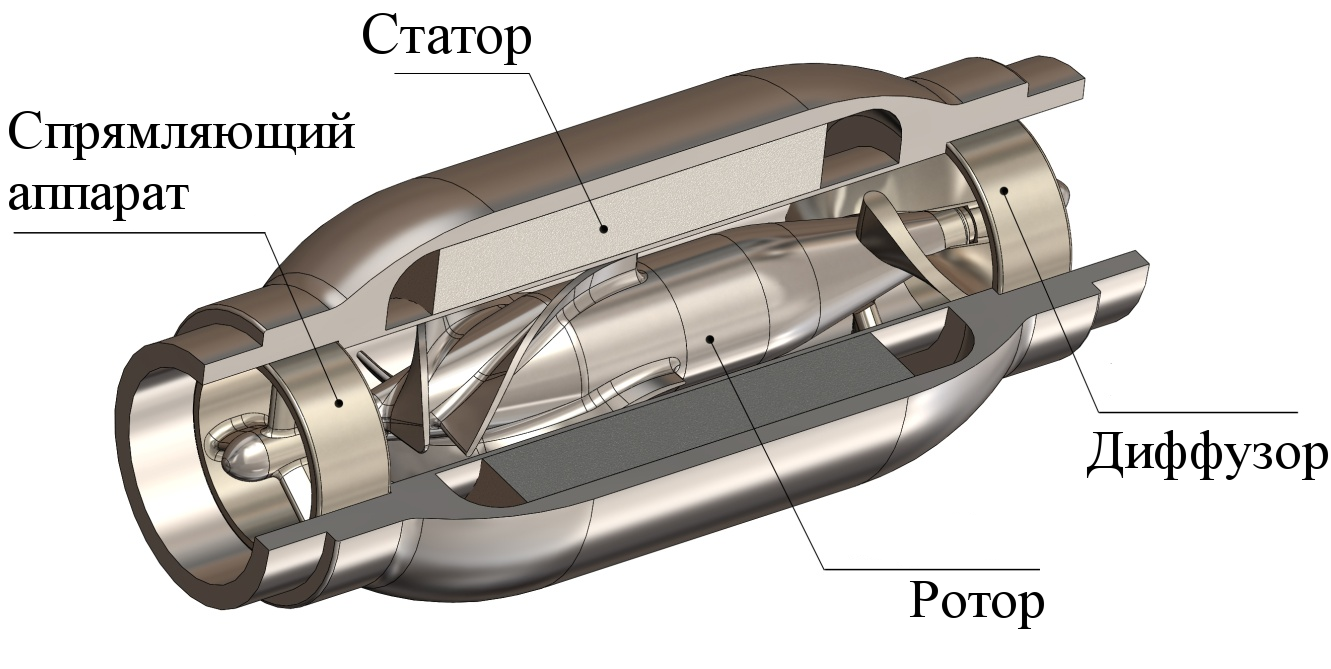
\includegraphics [width=0.6\textwidth] {../images/c1_sputnik_flow_part}
%   \caption{Проточная часть роторного насоса крови Спутник} 
%   \label{img:pump_view}  
% \end{figure}


\begin{figure}[ht]
%\fbox{
  \begin{minipage}[ht]{0.54\linewidth}
    \center{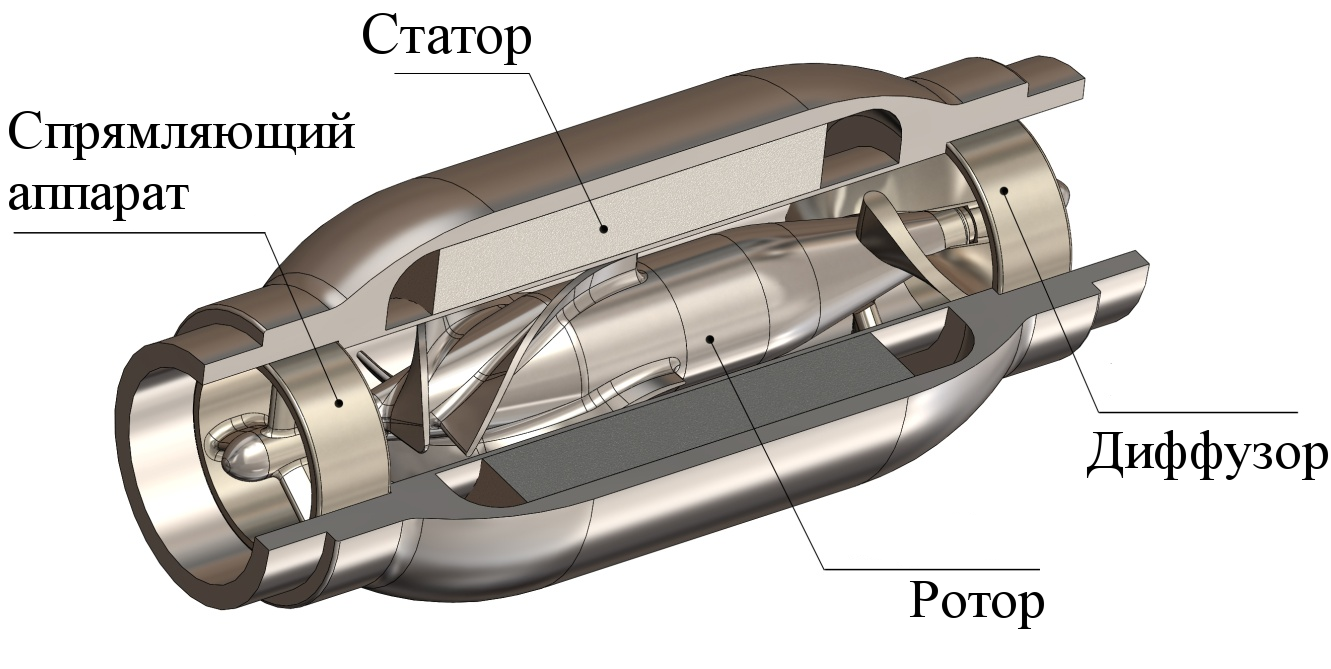
\includegraphics [scale=0.56] {../images/c1_sputnik_flow_part} \\ а)}
  \end{minipage} 
  \hfill
  \begin{minipage}[ht]{0.42\linewidth}
    \center{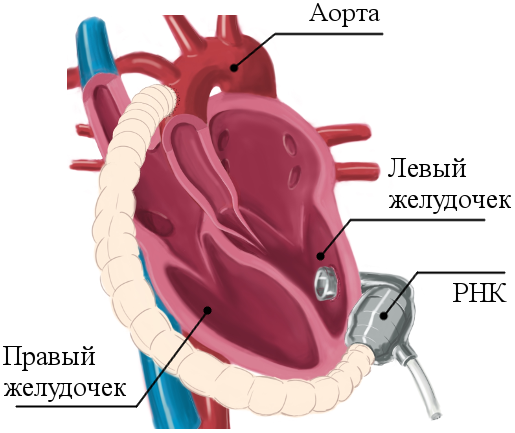
\includegraphics [scale=0.52] {../images/c1_pump_implantation_upd} \\ б)}
  \end{minipage}
  \caption{Проточная часть имплантируемого роторного насоса крови (а) и схема подключения насоса для поддержки кровообращения левого желудочка сердца (б)}
  \label{img:pump_view}  
\end{figure}

Роторные насосы крови, как правило, используются для поддержки кровообращения левого желудочка сердца. В этом случае входная канюля насоса подключается к левому желудочку сердцу, выходная -- к аорте -- рисунок \ref{img:pump_view}б. 

Первым роторным насосом, успешно применяемым в клинических условиях, стал Hemopump -- разработка Ричарда Вамплира, впервые имплантированная в 1988 году при участии доктора Фрейзера \cite{frazier2017invited}. Данный насос продемонстрировал возможность долговременной поддержки кровообращения при непульсирующем потоке крови через насос. Впоследствии на основе Hemopump был разработан роторный насос крови HeartMate II. 

В современной клинической практике представлено множество роторных насосов крови \cite{Patel2014667}. С 2000-го года имплантировано более 30 тысяч насосов, продолжительность поддержки кровообращения достигла 10 лет. Их широкое распространение обусловлено малыми массогабаритными параметрами, высокой надежностью и минимальной степенью гемолиза и тромбоэмболических осложнений. Среди наиболее известных и широко используемых роторных насосов крови следует выделить насосы Jarvik, HeartMate и HeartWare \cite{frazier2017invited, intermacs2017}. 

В результате рассмотрения исторического развития имплантируемых роторных насосов крови была подготовлена обзорная статья для журнала <<Медицинская техника>> \cite{mt6_2014}. Помимо роторных насосов крови, обеспечивающих частичную поддержку кровообращения, в современной клинической практике представлены аппараты для полной замены функции биологического сердца -- полностью искусственные сердца. Результаты обзора данных аппаратов, а также перспективы развития данной технологии были опубликованы в работах \cite{mt4_2015, mt5_2015}.

\subsubsection*{Jarvik 2000}

Разработка Jarvik 2000 началась в 1988 году при участи Jarvik Heart Inc. и Texas Heart Institute (THI). В апреле 2000 года в THI начались испытания Jarvik 2000 в качестве моста к трансплантации, а в марте 2005 был получен допуск Управления по санитарному надзору за качеством пищевых продуктов и медикаментов, мае 2005 года получен знак соответствия европейским стандартам качества (CE mark). 

Роторный насос Jarvik с осевым направлением течения, представленный на рисунке \ref{img:diff_pumps}а, имплантируется через подшиваемую манжету в левый желудочек сердца. Размеры насоса 2,5 см в ширину и 5,5 см в длину, вес -- 85 грамм. Внутри титанового корпуса насоса находится ротор, который представляет собой неодимий-ферроборовый магнит с титановыми лопатками, удерживаемый с помощью керамических подшипников. Скорость вращения ротора может изменяться от 8000 до 12000 об/мин, обеспечивая расход до 8 л/мин \cite{Westaby13101998, Healy20151794, Jarvik_cone_bearing_2013}. Одним из необходимых требований к имплантации Jarvik является площадь поверхности тела пациента не менее 1,2 м$^2$ (для сравнения нормальное значение для взрослых 1,73 м$^2$, для детей 12-13 лет -- 1,33 м$^2$).

%Система управления насосом позволяет изменять скорость вращения ротора вручную, либо автоматически с изменяемой длительностью импульсов. Комплект батарей обеспечивает до 8 часов бесперебойной работы. 

\subsubsection*{Incor}

Имплантируемый роторный насос Incor (Berlin Heart Inc., Германия) представлен на рисунке \ref{img:diff_pumps}б. 

Вес насоса составляет 200 грамм, длина -- 12 см, диаметр -- 3 см. Скорость вращения ротора насоса может изменяться от 5 до 10 тысяч об/мин, обеспечивая расход насоса до 7 л/мин. Контактирующие с кровью поверхности покрыты слоем гепарина по специальной технологии Carmeda BioActive Surface. Данный насос также обладает системой датчиков, позволяющей измерять перепад давления в насосе, что при известной скорости вращения ротора и геометрии насоса позволяет очень точно определить его расход \cite{Schmid20051188, Hetzer01062004}. 

%Система управления отображает и позволяет изменять параметры насоса. Комплект батарей обеспечивает до 12 часов бесперебойной работы.

\subsubsection*{DuraHeart}

Данный насос центробежного типа, представленный на рисунке \ref{img:diff_pumps}в, разработан компанией Terumo Heart, Inc. (США) для долговременной поддержки кровообращения. Насос состоит из двух титановых камер: в первой находятся позиционные сенсоры и ротор, во второй – бесколлекторный двигатель, который вращает ротор посредством индуктивной связи. 

Вес насоса составляет 540 грамм, диаметр -- 7,2 см, толщина -- 45 мм. Контактирующие с кровью поверхности насоса имеют гепариносодержащее покрытие. Скорость вращения ротора можно изменять в диапазоне от 1200 до 2400 об/мин, что позволяет обеспечить расход до 8 л/мин.

В настоящее время насос может имплантироваться в США в исследовательских целях \cite{DuraHeart, Morshuis01062009}.

% \begin{figure}[ht] 
%   \center
%   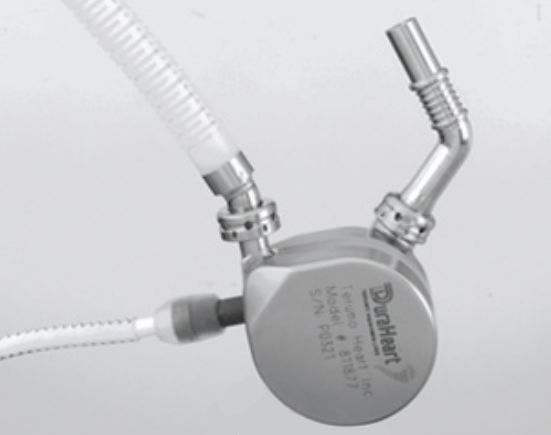
\includegraphics [width=0.6\textwidth] {../images/c1_duraheart_pump}
%   \caption{Роторный насос крови DuraHeart \cite{Morshuis01062009}} 
%   \label{img:duraheart_pump}  
% \end{figure} 

\begin{figure}[ht]
  \begin{minipage}[ht]{0.32\linewidth}
    \center{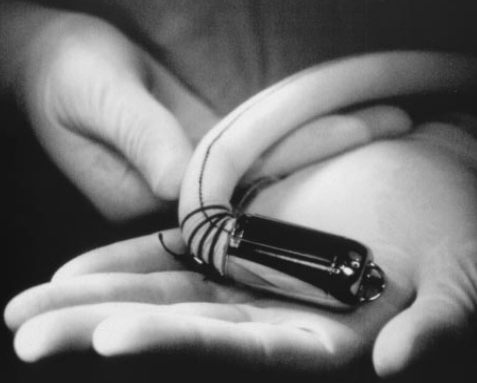
\includegraphics [scale=0.5] {../images/c1_jarvik_pump} \\ а)}
  \end{minipage}
  \hfill
  \begin{minipage}[ht]{0.32\linewidth}
    \center{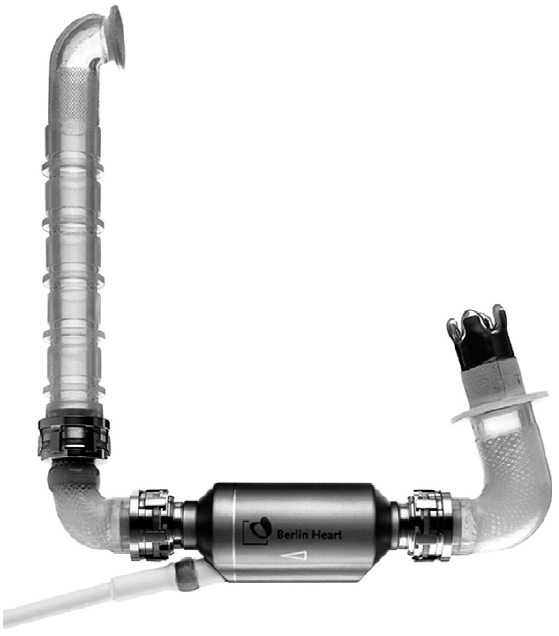
\includegraphics [scale=0.4] {../images/c1_incor_pump} \\ б)}
  \end{minipage}
  \hfill
  \begin{minipage}[ht]{0.32\linewidth}
    \center{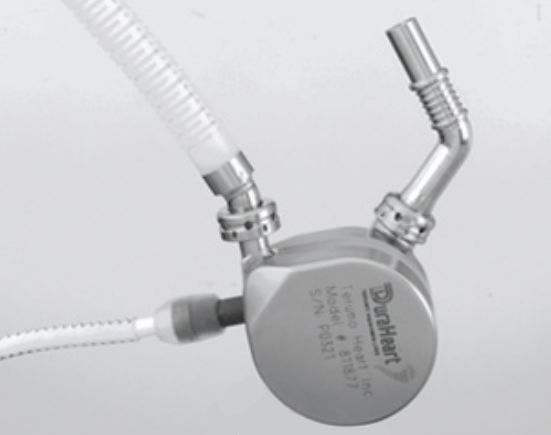
\includegraphics [scale=0.45] {../images/c1_duraheart_pump} \\ в)}
  \end{minipage}
  \caption{Роторные насосы крови Jarvik (а) \cite{Frazier2001S125}, Incor (б) \cite{Nakashima2009199} и DuraHeart (в) \cite{Morshuis01062009}}
  \label{img:diff_pumps}  
\end{figure}

\subsubsection*{ReliantHeart aVAD}

Разработка данного насоса началась в 1988 году при участи доктора Дебейки, инженеров из NASA и Бейлорского медицинского колледжа. В ноябре 1998 года в Берлине проведена первая имплантация. В апреле 2001 получен знак соответствия европейским стандартам качества, в феврале 2004 получен допуск Управления по санитарному надзору за качеством пищевых продуктов и медикаментов.

Обновленная версия насоса под названием HeartAssist5 \cite{HeartAssistFlow} получила знак соответствия европейским стандартам в мае 2009 года. В настоящее время данный роторный насос известен под названием ReliantHeart aVAD.

Роторный насос aVAD (ReliantHeart Inc., США) с осевым направлением течения позволяет обеспечить расход до 6 л/мин. Ротор насоса содержит шесть лезвий и вращается со скоростью 7500-12500 об/мин. Диаметр насоса -- 38 мм, длина -- 71 мм, вес -- 92 грамм. aVAD является единственным насосом, обладающим датчиком расхода на выходной канюле. Энергопотребление насоса составляет 10 Вт, продолжительность работы от батарей до 10 часов \cite{Loforte2017}. 

% \begin{figure}[ht] 
%   \center
%   \includegraphics [width=0.6\textwidth] {../images/c1_avad_pump}
%   \caption{Роторный насос крови ReliantHeart aVAD} 
%   \label{img:avad_pump}  
% \end{figure}

%Таким образом, суммарное время работы системы без подзаряда батарей составляет 5-8 часов. Система управления обладает функциональным набором, схожим с системой HeartWare.

\subsubsection*{HeartMate}

Наиболее часто имплантируемым роторным насосом с осевым направлением течения является HeartMate II (Thoratec Corp., США), представленный на рисунке \ref{img:heartmate_pumps}а. С момента выхода этой системы со стадии клинических испытаний в начале 2000-х годов по всему миру было имплантировано более 10 тысяч таких насосов \cite{frazier2017invited}.

\begin{figure}[ht]
  \begin{minipage}[ht]{0.48\linewidth}
    \center{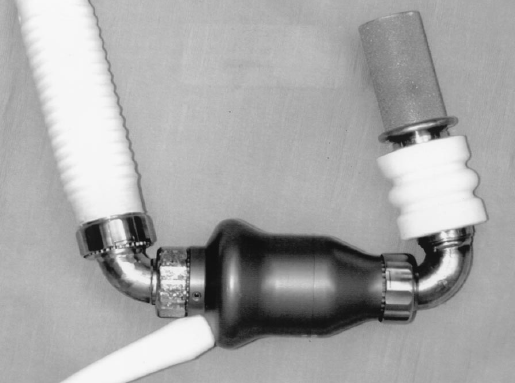
\includegraphics [scale=0.65] {../images/c1_heartmate_2_pump} \\ а)}
  \end{minipage}
  \hfill
  \begin{minipage}[ht]{0.48\linewidth}
    \center{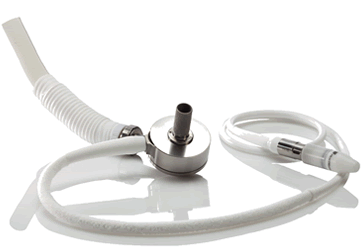
\includegraphics [scale=0.60] {../images/c1_heartmate_3_pump} \\ б)}
  \end{minipage}
  \caption{Роторные насосы крови HeartMate II (а) \cite{Griffith_2001} и HeartMate III (б) \cite{molina2013current}}
  \label{img:heartmate_pumps}  
\end{figure}

В ноябре 2005 года насос получил знак соответствия европейским стандартам качества, в апреле 2008 года -- допуск Управления по санитарному надзору за качеством пищевых продуктов и медикаментов \cite{HeartMate_II_Sheikh}. 

Вес насоса составляет 350 грамм, диаметр около 4 см и длина -- 7 см. Внутри насоса находится ротор, вращающийся посредством электродвижущей силы, генерируемой мотором. Скорость насоса может изменяться от 6000 об/мин до 15000 об/мин, обеспечивая поток крови до 10 л/мин \cite{Loforte20091357}. Время бесперебойной работы от аккумуляторов составляет около четырех часов \cite{Griffith_2001}. 

Обновленная версия насоса разработана компаниями Thoratec Corporation Inc. и Levitronix GmbH, называется HeartMate III (рисунок \ref{img:heartmate_pumps}б). Размеры насоса составляют 6,9 см в диаметре и 3 см в толщину, вес -- 500 грамм \cite{farrar2007design}. Ключевой особенностью данного насоса являются текстурированная внутренняя поверхность, уменьшающая требования к использованию антикоагулянтов, а также режим создания искусственных пульсаций потока и возможность косвенной оценки расхода с использованием собственных параметров насоса \cite{heartmate_speed_modulations, Schumerehv590}. Предполагается, что искусственные пульсации уменьшают не только вероятность образования тромбов, но и энергопотребление насоса. 

\subsubsection*{HeartWare}

Компания HeartWare Inc. (США) выпускает два роторных насоса крови центробежного типа -- HVAD и MVAD, представленных на рисунке \ref{img:heartware_pumps} \cite{larose2010design, cheung2015design}.
 
\begin{figure}[ht]
  \begin{minipage}[ht]{0.48\linewidth}
    \center{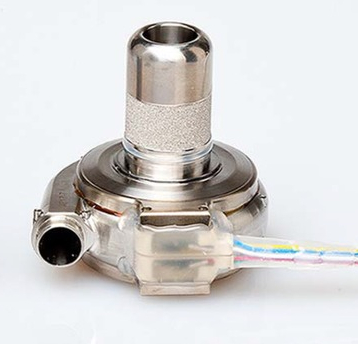
\includegraphics [scale=1.2] {../images/c1_hvad_pump} \\ а)}
  \end{minipage}
  \hfill
  \begin{minipage}[ht]{0.48\linewidth}
    \center{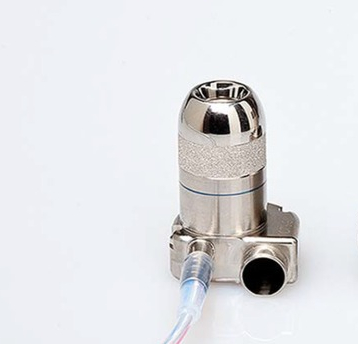
\includegraphics [scale=1.2] {../images/c1_mvad_pump} \\ б)}
  \end{minipage}
  \caption{Роторные насосы крови HVAD (а) и MVAD (б) \cite{cheung2015design}}
  \label{img:heartware_pumps}  
\end{figure}

На сегодняшний день HVAD является одним из наиболее широко используемых роторных насосов центробежного типа \cite{chorpenning2014heartware, rich2017hvad}. В январе 2009 года данный насос получил знак соответствия европейским стандартам (CE mark), в ноябре 2011 был получен допуск Управления по санитарному надзору за качеством пищевых продуктов и медикаментов для использования HVAD в качестве моста к трансплантации \cite{Carrel01012013}. 

Входная канюля данного насоса вставляется в левый желудочек сердца аналогично насосу Jarvik. В HVAD используются магнитные и гидродинамические опоры рабочего колеса, благодаря чему оно не изнашивается в процессе работы. Рекомендованная скорость вращения ротора данного насоса изменяется в пределах от 2400 до 3200 об/мин, обеспечивая расход 3,5-8 л/мин при энергопотреблении от 2,5 до 8,5 Вт, вес насоса составляет 160 грамм.

Роторный насос крови MVAD характеризуется меньшими размерами и весом (78 грамм). Скорость вращения ротора изменяется в пределах от 8 до 18 тысяч об/мин, обеспечивая расход до 7 л/мин. В настоящее время MVAD находится на этапе клинических испытаний \cite{cheung2015design}.

\subsubsection*{Спутник}

В настоящее время роторный насос крови Спутник, представленный на рисунке \ref{img:sputnik_pumps}а, успешно применяется в клинических условиях \cite{selishchev2015ventricular}. Имеет осевое направление течения, диаметр насоса составляет 35 мм, длина -- 82 мм, вес - 246 грамм, энергопотребление -- 8 Вт, скорость вращения ротора может изменяться от 5 до 10 тысяч об/мин.

\begin{figure}[ht]
  \begin{minipage}[ht]{0.48\linewidth}
    \center{\includegraphics [scale=0.235] {../images/c1_s1} \\ а)}
  \end{minipage}
  \hfill
  \begin{minipage}[ht]{0.48\linewidth}
    \center{\includegraphics [scale=0.235] {../images/c1_s2} \\ б)}
  \end{minipage}
  \caption{Имплантируемые роторные насосы крови Спутник первого (а) и второго поколений (б)}
  \label{img:sputnik_pumps}  
\end{figure}

Насос первого поколения был имплантирован 9 июня 2012 года 67-летнему пациенту с последующей успешной трансплантацией сердца. На сегодняшний день произведено более тридцати имплантаций насоса.

Помимо этого разрабатывается улучшенная версия насоса -- Спутник 2, представленная на рисунке \ref{img:sputnik_pumps}б. В данной версии диаметр был уменьшен до 29 мм, длина -- до 66 мм, энергопотребление было уменьшено на 15\%, масса -- до 205 грамм \cite{sputnik_upd}. В настоящее время проводятся испытания насоса на животных.

%Отмечается, что АВК Спутник в 2 раза дешевле заграничных аналогов, при этом он не уступает им в качестве и надежности \cite{lvad_ru}.

\section{Сравнительный анализ способов идентификации имплантируемых роторных насосов крови}\label{identification_review}

Таким образом, в современной клинической практике существует огромный выбор имплантируемых роторных насосов крови.

В то же время данные насосы пассивно реагируют на изменение состояния сердечно-сосудистой системы, что может приводить к коллапсу желудочка сердца, аритмии, отеку легких и внутренним кровотечениям \cite{tchantchaleishvili2017clinical, bozkurt2015physiologic,giridharan_hemodynamic_2015,mahr_intermittent_9000, aggarwal_incidence_2012, wever_pulsatility_2013, vollkron_suction_2007,salamonsen_anatomy_2015}. Это создает существенные риски для пациента и ограничивает безопасность и производительность АВК. Кроме того, высокая рабочая скорость насоса может приводить к коллапсу желудочка сердца, а также увеличению вероятности гемолиза и тромбообразования \cite{Vollkron2006, vollkron_suction_2007,Ng_2013}. В то же время, малая скорость насоса может приводить к обратному течению через насос \cite{giridharan_hemodynamic_2015, bozkurt2015physiologic}. 

Одним из основных направлений развития технологии вспомогательного кровообращения является управление имплантируемым роторным насосом крови, направленное на преодоление указанных проблем и повышение эффективности лечения различных форм сердечной недостаточности \cite{schima_noninvasive_1992,schloglhofer_international,JTD2878,Kyo2012101,lenneman2014treatment,Controller_review}.

На основе проведенного обзора алгоритмов управления имплантируемым роторным насосом крови была подготовлена и опубликована статья в журнале <<Медицинская техника>> \cite{mt3_2016}.

Для управления имплантируемыми роторными насосами крови необходима идентификация, которая понимается как построение математической модели системы по результатам экспериментальных исследований \cite{identification_usa}. 

% На данный момент предложено множество различных способов управления имплантируемым роторным насосом крови \cite{bozkurt2015physiologic,walter2012control,Controller_review,amacher2014synchronized,tchantchaleishvili2017clinical, moscato2010left}. Так, в работе S. Bozkurt \cite{bozkurt2015physiologic} описывается алгоритмы управления скоростью вращения ротора насоса, в том числе посредством задания профилей скорости. В работе M. Walter и др. \cite{walter2012control} рассматриваются общие принципы управления в биомедицинских применениях применительно к имплантируемым РНК. Наиболее полный обзор различных способов управления РНК представлен в работе AlOmari и др. \cite{Controller_review}. 

%Таким образом, на сегодняшний день разработано множество роторных насосов крови для управления которыми необходима идентификация. 

Обзор различных способов идентификации имплантируемого роторного насоса крови представлен в работах C. Bertram и A. AlOmari \cite{bertram2005measurement, Controller_review}. Построенные в результате идентификации математические модели используются при управлении системой и предсказания поведения идентифицируемой системы в будущем \cite{identification_usa}. 

В случае с роторными насоса крови построенные в результате идентификации математические модели могуть быть использованы для оценки физиологических параметров в сердечно-сосудистой системе с имплантированным насосом -- таких как,  перепад давления в насосе, давление в аорте, расход насоса и т.\:д. Полученные качественные и количественные данные о взаимодействии насоса и сердечно-сосудистой системы могут быть использованы для управления имплантируемым РНК. 

Так в системе управления HeartWare HVAD используется алгоритм оценки расхода насоса на основе таблиц о соотношении энергопотребления и расхода насоса, которые получены в результате экспериментального исследования насоса в испытательном гидродинамическом стенде \cite{reyes2016accuracy}. 

В работе F. Moscato и др. по идентификации разработана математическая модель на основе результатов экспериментального исследования РНК Micromed DeBakey \cite{Moscato_2009}. Разработанная модель описывается следующим уравнением:

\begin{equation}
	H(t) = \alpha \omega(t)^2 - \left[ aQ(t) + bQ(t)^2 \right] - L\frac{dQ(t)}{dt},
	\label{eq:moscato_equation}
\end{equation}

\noindent где $H(t)$ -- перепад давления в насосе, $\omega(t)$ -- скорость вращения ротора насоса, $Q(t)$ -- расход насоса, $\alpha$ -- параметр, связанный со скоростью вращения ротора, $a$ и $b$ -- параметры, характеризующие гидравлическое сопротивление, $L$ -- параметр, характеризующий инерцию жидкости в насосе. В работе продемонстрировано влияние инерции жидкости на расходно-напорную характеристику насоса, сделаны выводы о необходимости включения члена $LdQ/dt$ в уравнение, что позволяет улучшить точность оценки расхода насоса в пульсирующих условиях.

В работах T. Pirbodaghi предлагаются математические модели, разработанные на основе результатов исследований в испытательном гидродинамическом стенде \cite{Pirbodaghi_2011, Pirbodaghi_2017}. Пример математической модели согласно \cite{Pirbodaghi_2017} приводится далее: 

\begin{equation}
	H(t) = b_0Q(t) + b_1Q(t)^2 + b_2\omega(t)^2 + b_3\frac{dQ(t)}{dt} + b_4\frac{d\omega(t)}{dt},
	\label{eq:pirbodaghi_equation}
\end{equation}

\noindent где $H(t)$ -- перепад давления в насосе, $Q(t)$ -- расход насоса, $\omega(t)$ -- скорость вращения ротора насоса, $t$ -- время, $b_i$ -- коэффициенты уравнения. Указано, что добавление производных по времени позволяет увеличить точность описания работы насоса в пульсирующих условиях. 

В работе M. Granegger и др. разработана математическая модель с целью оценки расхода центробежного насоса на основе результатов исследования в гидродинамическом стенде при различных величинах вязкости жидкости \cite{Granegger_2012}. Модель описывается следующим уравнением:

\begin{equation}
	Q = aI + bI^2 + cI^3 + d\omega + e\omega^2 + g\omega I + h\omega^2 I + k - m\frac{d\omega}{dt},
	\label{eq:granegger_equation}
\end{equation}

\noindent где $Q$ -- расход насоса (л/мин), $I$ -- электрический ток (А), $\omega$ -- скорость насоса (об/мин), $a-m$ -- коэффициенты, заданные линейной функцией вида $x(\mu) = x_1\mu + x_2$, где $\mu$ -- вязкость жидкости (мПа$\cdot$с). Разработанная математическая модель характеризуется средней ошибкой при оценке расхода равной 0,06$\pm$0,31 л/мин и может быть использована для оценки сократительной способности желудочка сердца. 

В работе Г. Иткина разработаны математические модели на основе результатов исследований в испытательном гидродинамическом стенде \cite{vest_2015}. Разработанные математические модели предназначены для оценки расхода и перепада давления в насосе. Так, среднее значение расхода насоса рассчитывается согласно следующей формуле:

\begin{eqnarray}
	F_{PUMP} = K_1 + K_2\omega_{MEAN} + K_3\omega_{MEAN}^2 + K_4I_{MEAN} + K_5I_{MEAN}^2 + \nonumber \\ + K_6I_{MEAN}^3,
	\label{eq:itkin_equation}
\end{eqnarray}

\noindent где $F_{PUMP}$ -- среднее значение расхода насоса, $\omega_{MEAN}$ -- среднее значение скорости вращения ротора, $I_{MEAN}$ -- среднее значение электрического тока двигателя насоса, $K_1$, $K_2$, $K_3$, $K_4$, $K_5$ и $K_6$ -- коэффициенты. 

Также с целью оценки расхода насоса в работе E. Lim разработана математическая модель насоса, описываемая следующим уравнением \cite{Lim_2011}:

\begin{eqnarray}
	Q_p(k\tau) = 0,2710f([k-1]\tau) - 0,2546f([k-2]\tau) - 1,985Q_p([k-1]\tau) - \nonumber \\ - 1,240Q_p([k-2]\tau) - 0,2397Q_p([k-3]\tau) + e_1(k\tau),
	\label{eq:dynamic_model_lim}
\end{eqnarray}

\noindent где $Q_p$ -- расход насоса, $\tau$ -- интервал измерения равный 0,02 с, $e_1(k\tau)$ -- погрешность, $f$ -- функция, которая описывается следующим выражением:

\begin{equation}
	f = a_1 + a_2P + a_3P^2 + a_4P^3 + a_5\omega + a_6\omega^2,
\end{equation}

\noindent где $P$ -- потребляемая мощность, $a_1 - a_6$ -- коэффициенты, величина которых зависит от вязкости крови. Разработанная модель предназначена для использования в алгоритме управления расходом имплантируемого роторного насоса крови \cite{Lim_2011}. 

В работах Y. Wang и др. предлагаются математические модели насосов, предназначенные для управления расходом насосов \cite{wang2015rotary, wang2015suction}. Математические модели описываются следующими уравнениями:

\begin{equation}
	\frac{dF_p}{dt} = \frac{b_0}{b_1}F_p - \frac{b_2}{b_1}\omega^2 + \frac{1}{b_1}\Delta P,
	\label{eq:wang_equation_1}
\end{equation}

\begin{equation}
	J\frac{d\omega}{dt} = \frac{3}{2}K_BI - B\omega - a_0\omega^3 - a_1F_p\omega^2,
	\label{eq:wang_equation_1_speed}
\end{equation}

\noindent где $F_p$ -- расход насоса, $\omega$ -- скорость вращения ротора насоса, $\Delta P$ -- перепад давления в насосе, $J$ -- инерция ротора, $K_B$ -- постоянная противо-ЭДС, $I$ -- амплитуда фазового тока, $a_0$, $a_1$, $b_0$, $b_1$ и $b_2$ -- постоянные, определяемые экспериментально.

\begin{equation}
	\phi\frac{dF_p}{dt} = K_2\omega^2 - \Delta P - c_1\omega F_p - c_2\omega F_{p}^{2},
	\label{eq:wang_equation_2}
\end{equation}

\begin{equation}
	J\frac{d\omega}{dt} = K_1I - c_3\omega - c_4\omega F_p - T_R \frac{\omega}{\omega_{full}},
	\label{eq:wang_equation_2_speed}
\end{equation}

\noindent где $F_p$, $\omega$, $\Delta P$ и $J$ -- определены выше, $\phi$ -- параметр, характеризующий инерционные эффекты в насосе, $K_1$ -- коэффициент момента двигателя постоянного тока, $I$ -- электрический ток двигателя, $T_R$ -- коэффициент кинетического трения, $\omega_{full}$ -- скорость вращения ротора при полной разгрузке желудочка сердца, $K_2$, $c_1$, $c_2$, $c_3$ и $c_4$ -- параметры, зависящие от вязкости жидкости. 

Разработанные математические модели насосов исследованы на модели сердечно-сосудистой системы, продемонстрировав возможности поддержания физиологического расхода и предотвращения коллапса желудочка сердца.

В работе \cite{pennings2015estimation} разработана математическая модель по результатам исследований имплантируемых роторных насосов крови Micromed DeBakey и HeartMate II в испытательном стенде. Разработанная математическая модель предназначена для оценки давления в левом желудочке сердца и описывается следующим выражением:

\begin{eqnarray}
	P_{lv} = P_{ao} + dP_{out} - dP_{VAD},
	\label{eq:lv_pressure_estimation_pennings}
\end{eqnarray}

\noindent где $dP_{out}$ -- среднее аортальное давление, $dP_{VAD}$ -- средний перепад давления в насосе, рассчитываемый согласно следующей формуле:

\begin{equation}
	dP_{VAD}(t) = b_1Q_{VAD}(t) + b_2Q_{VAD}^{2}(t) + b_3n^2 + b_4\frac{dQ_{VAD}(t)}{dt} + dP_{hydro},
\end{equation}

\noindent где $b_1$, $b_2$, $b_3$ и $b_4$ -- коэффициенты, $Q_{VAD}$ -- расход насоса, $n$ -- скорость вращения ротора, $dP_{hydro}$ -- поправочный коэффициент, введенный из-за разницы в высоте датчиков давления левого желудочка сердца и давления на выходе насоса.

В работе \cite{hijikata2015estimating} разработана математическая модель центробежного насоса крови, предназначенная для оценки расхода насоса. Модель описывается следующим выражением:  

\begin{equation}
	Q = a'\frac{T}{n} + (b_1\mu + b_0)n + c_1\mu + c_0,
	\label{eq:hijikata_equation}
\end{equation}

\noindent где $T$ -- крутящий момент двигателя, $a'$, $b_0$, $b_1$, $c_0$ и $c_1$ -- коэффициенты, определенные экспериментально в испытательном гидродинамическом стенде,  $n$ -- скорость вращения ротора и $\mu$ -- вязкость рабочей жидкости. В ходе исследований в стенде с использованием воды абсолютная ошибка при оценке расхода не превысила 0,51 л/мин в диапазоне расхода насоса от 0 до 10 л/мин. В ходе исследований в стенде с использованием вязкой жидкости абсолютная ошибка составила менее 0,77 л/мин в аналогичном диапазоне расхода насоса.

% добавить критику работ, сделанных до меня (не приводятся алгоритмы идентификации, рассматриваются только результаты идентификации или возможности управления, которые реализованы в ходе решения задачи идентификации -- в иных условиях подход к управлению на основе данного подхода может не работать, только задача идентификации решена локально, а идентифицированная система не исследована в широком диапазоне)
% таблицы HVAD тоже идентификация, но без разработки математической модели, работа Salamonsen о преднагрузке тоже простая идентификация на основе подбора полинома, но без управления; Moscato -- нет алгоритма, добавление членов произвольно

Примеры различных математических моделей имплантируемых роторных насосов крови можно найти в работах \cite{bioengineering1010022, Moscato_2009, moscato2012evaluation, Pirbodaghi_2011, Pennings_2013, wang2015rotary, wang2015suction, alomari2011non, alomari2009non, gao2012pulsatile, Bakouri_2014, wu2009adaptive, Malagutti_2007, 4352467, Giridharan2003, simaan2009dynamical, choi2007hemodynamic, lim2008noninvasive, yoshizawa2002sensorless, kitamura2000physical, xu2000computer, takami1997flow, ayre2000sensorless}. %(не описывают как было разработано),

Следует отметить, что общим недостатком рассмотренных способов построения математических моделей имплантируемых роторных насосов крови является отсутствие универсального и общепринятого алгоритма. На построение математической модели оказывает влияние геометрия ротора насоса \cite{ayre2000sensorless}, таким образом разнообразие конструкций роторных насосов крови создает потребность в разработке универсального алгоритма идентификации. При идентификации также необходимо учитывать взаимодействие насосов с сердечно-сосудистой системой. 

% ----------------------------------------------------------------------------------------------------------------------------------------------------------------------------------------------------------------------------
% ----------------------------------------------------------------------------------------------------------------------------------------------------------------------------------------------------------------------------

%Отличие данной работы заключается в рассмотрении систем управления аппаратами вспомогательного кровообращения, которые находят применение в современной клинической практике \cite{Mancini_2015,Patel2014667}. При их рассмотрении использовались как результаты обзора патентов соответствующих компаний \cite{brown2015methods,larose2005sensorless, tamez2014vad, yomtov2015physiologically, bourque2015generating, yanai2014backflow, medvedev2016method}, так и данные, опубликованные в литературе \cite{reyes2016accuracy, chorpenning2014heartware, cheung2015design, Healy20151794, Slaughter2010S1, lund2012derived, HeartAssistFlow}. Основное внимание уделено обзору систем, методов и алгоритмов управления, опубликованных в литературе за последние пять лет. 

%Исходно предлагается следующая классификация: методы и алгоритмы оценки и регулирования расхода насоса, определения и управления режимами работы роторного насоса крови, и физиологического управления. К первым относятся методы и алгоритмы оценки расхода насоса \cite{hijikata2015estimating, Granegger_2012,vest_2015} и его регулирования с определенными целями \cite{Bozkurt20141288, Lim_2011}. Ко вторым относятся методы и алгоритмы определения состояния коллапса желудочка сердца \cite{Ng_2013, Ochsner_2013, 6359938}, состояния аортального клапана \cite{Jansen_Park01092014,Granegger_2014,Hui_2014,6944257,Hayward_2015,7295582,Ooi_2015,6862467,vest_2014} и управления данными состояниями. К третьим -- методы и алгоритмы физиологического управления, регулирующие работу насоса относительно некоторых физиологических параметров \cite{wang2015rotary, huang2014pulse,bioengineering1010022}, либо имитирующие механизм Старлинга \cite{6606105,6609590,Bakouri_2014,Salamonsen_2012,Mansouri_2015,Ochsner_2014}.

%\subsection*{Управление с постоянной скоростью насоса}

% Данный способ управления заключается в поддержании скорости вращения ротора насоса независимо от состояния сердечно-сосудистой системы либо регулировании скорости врачами в клинических условиях. В то же время, он характеризуется ограниченными возможностями для адаптации к потребностям сердечно-сосудистой системы \cite{Lim_2011, tchantchaleishvili2017clinical}. Так, роторные насосы крови уменьшают напор с увеличением расхода при постоянной скорости вращения ротора, в то время как физиологические потребности тела заключаются в увеличении расхода с увеличением давления. 

% Несмотря на это, система управления HeartAssist 5 (ReliantHeart Inc., США) позволяет поддерживать постоянную скорость вращения ротора насоса. Решение об изменении скорости вращения ротора принимается лечащим врачом на основе данных об измеренном расходе насоса, потребляемой мощности и скорости вращения ротора за последние 30 дней, которые доступны дистанционно на VADLink.com \cite{HeartAssistFlow}. 

% Описанные способы управления имплантируемыми роторными насосами крови требуют периодического посещения больницы и принятия решения лечащим врачом о регулировании скорости насоса. В то же время, система управления Jarvik 2000 (Jarvik Heart Inc., США) позволяет пациенту самостоятельно регулировать скорость вращения ротора насоса \cite{Healy20151794}. В зависимости от своего самочувствия или уровня физической активности пациент может выбирать значения в диапазоне от 1 до 5, что соответствует изменению скорости вращения ротора от 8000 об/мин до 12000 об/мин и может значительно изменять расход насоса. Предполагается, что постепенное уменьшение скорости должно обеспечить поступательное увеличение нагрузки на желудочек сердца и помочь восстановлению сердечной мышцы \cite{Healy20151794}. 

% Кроме того, в Jarvik 2000 применяется алгоритм, который уменьшает скорость вращения ротора до 7000$\pm$200 об/мин в течение 10 секунд каждую минуту. Предполагается, что это позволит уменьшить степень разгрузки левого желудочка сердца и увеличит вероятность выброса крови через аортальный клапан \cite{Jarvik_cone_bearing_2013, arndt_fully_2010}. Аналогичные алгоритмы управления разработаны для роторных насосов крови Incor (Berlin Heart GmbH, Германия) \cite{arndt_fully_2010} и HeartWare MVAD \cite{Kapur2013S53, cheung2015design}. Так, в MVAD применяется алгоритм  <<qPulse Cycle>>, который уменьшает скорость вращения ротора на 15\% или 20\% в течение 5 секунд с последующим увеличением скорости до исходного значения в течение 10-30 секунд. 
% 
% Следует отметить, что данный тип управления является общепринятым для имплантируемых роторных насосов крови, применяемых в клинической практике \cite{larose2010design, Slaughter2010S1, HeartAssistFlow, Healy20151794, advanced_development_2011,bozkurt2015physiologic}.

%\subsection*{Управление с переменной скоростью насоса}

% Данный тип управления имплантируемым роторным насосом крови позволяет автоматически по определенным правилам изменять скорость вращения ротора насоса. 

% Так, в патенте \cite{larose2005sensorless} описывается механизм управления скоростью вращения ротора, позволяющий поддерживать заданную величину расхода насоса. В работе E. Lim и др. \cite{Lim_2011} также предлагается алгоритм поддержания расхода насоса на заданном уровне. Аналогичный алгоритм управления расходом роторного насоса крови с возможностью предотвращения коллапса желудочка сердца представлен в работе \cite{simaan2009dynamical}.

% В роторном насосе крови HeartWare HVAD имеется возможность регулирования скорости вращения ротора насоса в случае обнаружения коллапса желудочка сердца \cite{brown2015methods, reyes2016accuracy, medvedev2016method}. В системе управления HeartWare MVAD также имеется алгоритм управления, реагирующий на возникновение коллапса желудочка сердца \cite{cheung2015design}. Данный алгоритм уменьшает скорость вращения ротора на 15\% с последующим увеличением до исходного значения. Если состояние коллапса не обнаруживается, то алгоритм выключается, в ином случае скорость вращения ротора уменьшается на 25\% с последующим увеличением до исходного значения. Описанный цикл повторяется до тех пор, пока состояние коллапса сохраняется.

% Подобные алгоритмы разработаны для роторных насосов крови VentrAssist \cite{mason2008reliable}, HeartMate II и Incor. Так, управление Incor заключается в поддержании заданной величины индекса пульсаций \cite{arndt_fully_2010}. Индекс пульсаций вычисляется на основе измеренного перепада давления в насосе и предназначен для предотвращения коллапса желудочка сердца.  

% %%% -----------------------------------------------------------------------------
% 
% В работе F. Moscato и др. предложен алгоритм управления скоростью роторного насоса крови на основе данных о давлении в левом желудочке сердца \cite{moscato2010left}. Давление в желудочке оценивается с помощью фильтра Калмана с увеличенной памятью и данных об аортальном давлении, расходе насоса и скорости вращения ротора. Предоженный алгоритм позволяет поддерживать определенный уровень нагрузки на желудочек сердца в различных физиологических условиях, что подтверждается исследованием на математической модели сердечно-сосудистой системы.

%%% -----------------------------------------------------------------------------

% В работе \cite{wang2015suction} предложен алгоритм управления скоростью вращения ротора насоса крови за счет поддержания фиксированной разности давления между левым желудочком и аортой. Предложенный алгоритм направлен на обеспечение физиологического расхода насоса и позволяет предотвратить коллапс желудочка сердца, что подтверждается результатами исследования на математической модели сердечно-сосудистой системы. Подобные алгоритмы управления с целью поддержания фиксированного перепада давления в насосе были предложены в работах \cite{waters1999, giridharan2002, giridharan2006}.
% 
% В работах \cite{Salamonsen_2012, Bakouri_2014} предлагается алгоритм управления скоростью вращения ротора на основе данных о величине пульсаций расхода насоса. Предлагаемый алгоритм позволяет установить равновесие между сердечным выбросом правого желудочка сердца и объединенным расходом левого желудочка и насоса, что позволяет предотвратить недостаточную и избыточную откачку крови из левого желудочка сердца. Аналогичные алгоритмы управления также представлены в работах \cite{Mansouri_2015, Ochsner_2014, petrou2016physiological, alomari2009non}. Так, в работе \cite{Mansouri_2015} управление скоростью осуществляется на основе данных о конечно-диастолическом давлении в левом желудочке сердца, в работе \cite{alomari2009non} -- на основе данных о скорости вращения ротора и потребляемой мощности. 

%%% -----------------------------------------------------------------------------

% В работе A. Arndt и др. предлагается алгоритм управления на основе градиента пульсационного индекса по скорости насоса \cite{Arndt_2008}. Пульсационный индекс рассчитывается с использованием перепада давления в насосе. Предлагаемый алгоритм позволяет роторному насосу крови функционировать в двух различных рабочих точках: частичная разгрузка желудочка сердца при поддержании заданной величины градиента или полная разгрузка желудочка с предотвращением коллапса посредством минимизации вычисленного градиента и максимизации пульсационного индекса. 

%К недостаткам алгоритма управления следует отнести медленную реакцию на изменения в преднагрузке, что делает необходимым применение отдельного алгоритма предотвращения коллапса желудочка сердца. Так, в случае коллапса происходит увеличение пульсационного индекса из-за увеличения пульсового давления, что требует от алгоритма управления увеличения скорости насоса и, следовательно, прогрессирования коллапса желудочка \cite{tchantchaleishvili2017clinical}.

% К управлению с переменной скоростью вращения ротора также относятся алгоритмы, модулирующие скорость вращения ротора насоса синхронно или асинхронно с сердечным циклом. Данные алгоритмы управления описаны в патентах компании HeartWare \cite{yomtov2015physiologically} и Thoratec \cite{bourque2015generating}. При этом учитывается наличие аритмий желудочка сердца \cite{yomtov2015physiologically}. Алгоритмы модулирования скорости вращения ротора реализованы в системе управления HeartMate III \cite{heartmate_speed_modulations, Schumerehv590}. Предполагается, что искусственные пульсации уменьшают вероятность образования тромбов, но, в то же время, приводят к большему энергопотреблению. 
% 
% В работе \cite{vandenberghe2005hemodynamic, bozkurt2016arterial} установлено, что управление синхронизированное с сердечным циклом приводит к увеличению ударного объема и уменьшению желудочкового давления, в то время как асинхронное управление создает давления и расходы, выходящие за пределы физиологического диапазона. В работе \cite{ising2011flow} установлено, что синхронное и асинхронное управление позволяет увеличить пульсовое давление. 

%%% -----------------------------------------------------------------------------

% В работе \cite{bioengineering1010022} описывается алгоритм получения профилей скорости, синхронизированных с сердечным циклом, который может оптимизировать взаимодействие роторного насоса крови и сердечно-сосудистой системы. Профиль скорости вращения ротора насоса задается с помощью следующей формулы:
% 
%  \begin{equation}
% 	\omega(t) = \omega_c + \omega_A \cdot \left( 2\pi (\gamma_c(t) + \varphi + 0,25)  \right),
% \end{equation}
% 
% \noindent где $\omega_A$ -- амплитуда в об/мин, $\varphi$ -- сдвиг по фазе приведенный к продолжительности одного сердечного цикла, $\gamma_c(t)$ -- периодический пилообразный сигнал, описывающий его распространение через каждый сердечный цикл. В качестве результатов приводятся профили скорости, синхронизированные с сердечным циклом, которые являются оптимальными по отношению к выбранной в данной работе цели управления -- максимизация потока через аортальный клапан и минимизация ударной работы. Предлагаемый алгоритм предназначен для разработки персонифицированных стратегий управления роторным насосом крови. Необходимость оптимизации параметров, определяющих профиль скорости подчерикивается в работе \cite{amacher2014synchronized}.

%%% -----------------------------------------------------------------------------

% В работе \cite{huang2014pulse} предложен алгоритм управления, который позволяет поддерживать среднее аортальное давление на уровне 100 мм рт. ст. и увеличить пульсовое давление до 20 мм рт. ст.. Для этого используются модуляция скорости вращения ротора на основе индексов, вычисленных из временной диаграммы аортального давления и позволяющих определить амплитуду модуляций и синхронизировать их с сердечным циклом. Алгоритм исследован на модели сердечно-сосудистой системы и в ходе предварительных \textit{in vitro} испытаний. Влияние модуляций скорости на аортальное давление и сравнение с режимом постоянной скорости представлено на рисунке \ref{img:speed_modulations_physio}.
% 
% \begin{figure}[ht] 
%   \center
%   \includegraphics [scale=0.8] {../images/c1_speed_modulations_physio}
%   \caption{Влияние режима модуляции скорости насоса и режима постоянной скорости насоса на аортальное давление \cite{huang2014pulse}}
%   \label{img:speed_modulations_physio}
% \end{figure}

% Все рассматриваемые режимы позволяют поддержать среднее аортальное давление на уровне 100 мм рт. ст., однако при постоянной скорости величина пульсового давления значительно уменьшается и становится меньше исходной величины пульсового давления, отмеченной точечной линией. В тоже время, модуляции скорости позволяют увеличить его до 20 мм рт. ст. с использованием профиля скорости прямоугольной формы \cite{huang2014pulse}.

%%% -----------------------------------------------------------------------------

% Алгоритм увеличения пульсаций расхода насоса и аортального давления посредством модуляции скорости вращения ротора насоса предложен в \cite{Bozkurt20141288}. При его разработке использовался гидродинамический стенд с изолированным свиным сердцем при частоте сердечных сокращений 140 уд/мин и насосом Micromed DeBakey. Продемонстировано, что увеличение пульсаций расходной характеристики приводит к увеличению пульсового давления. Таким образом, предложенный алгоритм позволяет удвоить индекс пульсаций по сравнению с режимом постоянной скорости при аналогичном уровне среднего аортального давления и расходе насоса \cite{Bozkurt20141288}.

% Результаты испытаний на гидродинамическом стенде представлены на рисунке \ref{img:speed_modulations_bozkurt}. В пульсирующем режиме амплитуда аортального давления больше, чем при постоянной скорости насоса; при этом в обоих режимах среднее артериальное давление составляло 80 мм рт. ст., средний расход -- 6,3 л/мин. Амплитуда измеренного расхода также примерно в два раза больше амплитуда расходной характеристики при постоянной скорости насоса. 
% 
% \begin{figure}[ht] 
%   \center
%   \includegraphics [scale=0.95] {../images/c1_speed_modulations_bozkurt}
%   \caption{Временные диаграммы аортального давления (слева) и расхода насоса (справа) в пульсирующем режиме (черная линия) и режиме постоянной скорости (серая линия) насоса \cite{Bozkurt20141288}}
%   \label{img:speed_modulations_bozkurt}
% \end{figure}
% 
% Постоянная рабочая скорость насоса составляла 9650 об/мин, для создания пульсирующего режима испытаний она варьировалась в диапазоне от 7200 до 12000 об/мин в течение одного сердечного цикла (средняя скорость около 9800 об/мин). 

%%% -----------------------------------------------------------------------------

% Так, в \cite{Ochsner_2013} исследуются индексы для определения коллапса желудочка сердца. Первый -- пульсационный индекс -- вычисляется следующим образом:
% 
% \begin{equation}
% 	PI = \frac{\max\left( x_{vad}(t) \right) - \min\left( x_{vad}(t) \right)}{2},
% 	\label{eq:pulsatility_index}
% \end{equation}
% 
% \noindent где $x_{vad}(t)$ может быть расходом насоса, электрическим током двигателя или перепадом давления в насосе. Гармонический индекс вычисляется следующим образом:
% 
% \begin{equation}
% 	HI = \frac{\int_{f_0-\delta f}^{f_0+\delta f} \! X_{vad}(f) \, \mathrm{d}f}{\int_{f_0+\delta f}^{f_{max}} \! X_{vad}(f) \, \mathrm{d}f},
% 	\label{eq:harmonic_index}
% \end{equation}
% 
% \noindent где $f$ -- частотная переменная, $f_0$ -- частота, соответствующая основной форме колебаний, т.\:е. частоте сердечных сокращений, $\delta f$ = 0,1 Гц -- постоянная частотного окна, $f_{max}$ = 80 Гц -- максимальная частота и $X_{vad}(f)$ -- величина дискретного преобразования Фурье для расхода насоса, электрического тока или перепада давления. 

% Результаты исследования индексов на гидродинамическом стенде представлены на рисунке \ref{img:suction_detection_m1}.
% 
% \begin{figure}[ht] 
%   \center
%   \includegraphics [scale=0.75] {../images/c1_suction_detection_m1}
%   \caption{Анализ изменений пульсационного и гармонического индексов при различных скоростях насоса \cite{Ochsner_2013}}
%   \label{img:suction_detection_m1}
% \end{figure}
% 
% Скорость вращения ротора насоса варьировалась в диапазоне от 3800 до 5800 об/мин с шагом 200 об/мин и фиксировалась в течении 30 секунд. Последние десять секунд записанных сигналов использовались для вычисления индексов с помощью формул \eqref{eq:pulsatility_index} и \eqref{eq:harmonic_index}. Изменение пульсационных индексов представлено слева, изменение гармонических индексов -- справа. Все шесть индексов имеют локальный минимум в случае возникновения коллапса желудочка сердца, т.\:е. с при скорости вращения ротора от 4800 об/мин и более.

% В работе \cite{6359938} описывается метод определения коллапса желудочка сердца, который рассматривает три состояния: нормальная работа насоса, приближение к коллапсу и работа в режиме коллапса желудочка сердца. Для определения данного состояния используется метод опорных векторов Лагранжа, который комбинирует шесть индексов, вычисленных из временной диаграммы расхода насоса. Примеры индексов, используемых в работе, приводятся ниже:
% 
% \begin{gather*}
% 	SI_1 = \frac{2\mathrm{mean}(PF) - (\max(PF)+\min(PF))}{\max(PF) - \min(PF)}, \\
% 	SI_2 = \frac{\max \left( \frac{d(PF)}{dt} \right) }{\max(PF) - \min(PF)}, \\
% 	SI_3 = \frac{\min \left( \frac{d(PF)}{dt} \right) }{\max(PF) - \min(PF)},
% 	\label{eq:wang_suction_indices}
% \end{gather*}
% 
% \noindent где $PF$ -- временная диаграмма расхода насоса, $d(PF)/dt$ -- производная расхода насоса по времени, $\mathrm{mean}$, $\max$ и $\min$ -- среднее, максимальное и минимальное значения соответственно. Данный метод был протестирован с использованием результатов \textit{in vivo} испытаний двух роторных насосов крови. 

% В работе \cite{Ng_2013} предложен 171 индекс для определения коллапса желудочка сердца на основе временной диаграммы скорости вращения ротора насоса. Данные индексы классифицированы следующим образом: амплитудные, временные, градиентные и частотные. Полученные индексы протестированы на данных, включающих различные режимы работы насоса, в том числе и данные с аритмией сердца. С использованием только двух индексов -- максимальное изменение градиента при положительном наклоне зависимости и стандартное отклонение максимального значения -- продемонстрирована чувствительность 98,9\% и специфичность 99,7\%.

% В работе \cite{Jansen_Park01092014} предложен метод определения момента закрытия АК на основе данных о площади циклической зависимости давления левого желудочка сердца от мощности, потребляемой насосом. Для ее расчета использовались результаты испытаний на животных. Изменение рассчитанной зависимости в диапазоне скоростей вращения ротора от 1000 об/мин до 2000 об/мин представлено на рисунке \ref{img:ano_detection}. 
% 
% \begin{figure}[ht] 
%   \center
%   \includegraphics [scale=1.0] {../images/c1_ano_detection}
%   \caption{Изменение интегрированной зависимости давления в левом желудочке сердца от мощности насоса при различных скоростях насоса \cite{Jansen_Park01092014}}
%   \label{img:ano_detection}
% \end{figure}
% 
% Показано, что полученная зависимость давления от мощности достигает максимума тогда, когда увеличение скорости вращения ротора насоса приводит к полностью закрытому состоянию АК. Авторы позиционируют свою работу в качестве основы для разработки контроллера автоматического управления, который будет предоставлять информацию о функции левого желудочка сердца и состоянии аортального клапана. 

% В настоящей работе исследуется производительность 14 индексов для определения такого состояния, полученных из временной диаграммы скорости насоса с использованием четырех различных типов классификаторов, включая линейный дискриминантный анализ, логистическую регрессию, нейронные сети с обратным распространением и алгоритм получения К-ближайший соседний результат. 
% Экспериментальные измерения от четырех гончих были использованы. Общая точность около 94.6\% \cite{Hui_2014}.

% Аппараты вспомогательного кровообращения (АВК) зарекомендовали себя как эффективное средство лечения тяжелых форм сердечной недостаточности наряду с трансплантацией сердца \cite{Patel2014667,Mancini_2015,HT_LVAD_2013,Lima2015360,Schumerehv590,ottenberg_choices_2014,selzman_bridge_2015,drakos_clinical_2016}. Множество пациентов с различными патологиями сердечной функции и широкий выбор АВК создает необходимость в различных подходах к лечению \cite{schima_noninvasive_1992,schloglhofer_international,JTD2878,Kyo2012101,lenneman2014treatment}. С целью разработки новых подходов к лечению, предотвращения физиологических нарушений, обусловленных спецификой работы роторного насоса крови, улучшения результатов лечения и качества жизни пациентов разрабатываются системы, методы и алгоритмы управления работой имплантируемых роторных насосов крови для аппаратов вспомогательного кровообращения. 

\section*{Выводы по главе 1} 
\addcontentsline{toc}{section}{Выводы по главе 1}

В данной главе рассмотрена история развития имплантируемых роторных насосов в аппаратах вспомогательного кровообращения, продемонстрировано многообразие имплантируемых роторных насосов крови, применяемых в современной клинической практике. 

Представлен аналитический обзор литературных источников, посвященных проблеме идентификации имплантируемых роторных насосов крови в аппаратах вспомогательного кровообращения -- т.\:е. проблеме построения математической модели насоса или процесса взаимодействия насоса с сердечно-сосудистой системой на основе результатов экспериментального исследования.

Рассмотрены различные структуры математических моделей, полученные в результате идентификации, описано применение математических моделей для управления имплантируемыми РНК в АВК. 

Как правило, работы по идентификации имплантируемых РНК направлены на повышение точности аппроксимации исходных экспериментальных данных математической моделью. Указано, что построенные в результате идентификации математические модели в общем случае применяются для управления расходом имплантируемого роторного насоса крови. 

Выявлено, что не существует универсального и общепринятого алгоритма идентификации, т.\:е. в каждом случае задача идентификации решается индивидуально для каждого насоса. Это обусловлено многообразием насосов, их сложным устройством, зависимостью производительности насосов от состояния сердечно-сосудистой системы, что требует учета взаимодействия насосов с сердечно-сосудистой системой при идентификации.

%В данной главе также проведен обзор различных способов управления имплантируемым роторным насосом крови в аппаратах вспомогательного кровообращения. Предложена следующая классификация: управление с постоянной скоростью и с переменной скоростью вращения ротора насоса. Рассмотрены основные направления развития данных типов управления, а также их ограничения. Так, недостатки управления с постоянной скоростью вращения ротора могут быть преодолены с помощью алгоритмов периодического уменьшения скорости либо алгоритмов управления коллапсом желудочка сердца, что требует оценки расхода насоса и определения состояния коллапса. Модулирование скорости насоса приводит к увеличению энергопотребления насоса и может потребовать синхронизации с сердечным циклом.

Таким образом, актуальной является задача идентификации имплантируемых роторных насосов крови с использованием универсального алгоритма. Для этого необходима структурная идентификация, которая требует представления объекта управления  в виде математической модели с определением ее структуры, и параметрическая идентификация, которая заключается в определении числовых значений коэффициентов математической модели согласно экспериментальным данным, с последующим исследованием и оценкой эффективности идентификации для управления имплантируемыми роторными насосами крови в аппаратах вспомогательного кровообращения.

С целью структурно-параметрической идентификации имплантируемых роторных насосов крови в диссертационной работе поставлены следующие задачи:

\begin{enumerate}
  \item Разработать математическую модель идентификации имплантируемого роторного насоса крови на основе расходно-напорных характеристик.
  \item Разработать математическую модель сердечно-сосудистой системы с учетом имплантации роторного насоса крови.
  \item Исследовать взаимодействие имплантируемого роторного насоса крови с сердечно-сосудистой системой методами математического моделирования.
  \item Исследовать взаимодействие имплантируемого роторного насоса крови с сердечно-сосудистой системой с использованием экспериментальных данных для роторных насосов крови Спутник.
\end{enumerate}

% Задаче идентификации имплантируемого роторного насоса крови посвящена \ref{chapt2}-я глава диссертационной работы. С целью исследования связей в сложной системе, образованной насосом, сердцем и сосудистой сетью, разрабатывается математическая модель сердечно-сосудистой системы с учетом имплантации роторного насоса крови. 
% 
% Последующее исследование и анализ взаимодействия насоса и сердечно-сосудистой системы методами математического моделирования позволяет оценить эффективность идентификации для управления имплантируемым роторным насосом крови -- данной задаче посвящена \ref{chapt3}-я глава диссертационной работы. 
% 
% Исследованию взаимодействия насоса и сердечно-сосудистой системы с использованием экспериментальных данных для отечественных имплантируемых роторных насосов крови Спутник посвящена \ref{chapt4}-я глава диссертационной работы.
% 
% Таким образом, набор основных требований, которым должны удовлетворять система управления имплантируемым роторным насосом крови, выглядит следующим образом: корректная оценка расхода роторного насоса крови (РНК), достижение и поддержание требуемого уровня расхода при различных физиологических условиях, определение и предотвращение неблагоприятных режимов работы РНК, обеспечение выбранной стратегии лечения, соответствие расхода РНК физиологическим потребностям организма.

